\begin{section}{Mise en place d'un bootstrapping}

Dans cette section, nous supposerons que $q$ est une puissance de 2, ne regarderons des chiffrés que de 0 ou 1.

Afin de pouvoir effectuer un bootstrapping à partir de l'algorithme de déchiffrement \textbf{Decrypt}, nous
allons avoir besoin de d'exprimer, pour tout chiffré $C$, l'algorithme de déchiffrement de $C$ comme 
un circuit booléen ayant pour entrée le chiffré de la clé secrète, pour cela préalablement représenté
uniquement à l'aide de 0 et de 1.

Nous allons donc créer ce circuit et nous trouverons une majoration de la profondeur de NAND qu'il nécessite afin de pouvoir, dans une dernière partie, trouver des paramètres sécurités permettant le bootstrapping.

Rappelons enfin que $l = \log_2(q)+1$ et que $N = (n+1)*l$.
\begin{subsection}{Un point sur la sécurité}
Nous avons vu que le système cryptographique que nous étudions est IND-CPA. 
La première question qui se pose pour le bootstrapping est de savoir si il a la sécurité
circulaire, expliquée dans la définition~\ref{def:circular}.  Nous n'avons pas trouvé de démonstration de cette sécurité
dans l'article original \cite{EPRINT:GenSahWat13} ou encore dans d'autres expositions (comme \cite{halevi}). Nous devons
donc la supposer pour cette section.
\end{subsection}
\begin{subsection}{Un premier découpage}
Comme la clé secrète est un vecteur de $\ZZq^N$ et qu'un élément de $\ZZq$ a une décomposition binaire d'au plus $\log_2(q)$ éléments, nous pouvons représenter la clé secrète par une liste de $N\log_2(q)$ 0 et 1.

L'algorithme que nous allons étudier est le suivant:
\begin{lstlisting}[label={lst:decoupage}]
decrypt(C) :
	trouver $1 \leqslant i \leqslant l$ tel que $q/4 \leqslant 2^i < q/2$
	calculer $a = C_i \cdot \vec{v}$
	retourner $|\frac{a}{\vec{v}_i}|$
\end{lstlisting}
Insistons sur le fait que le chiffré $C$ n'est pas une entrée du circuit. Notamment, même lors de 
l'application homomorphe de ce circuit, nous pouvons supposer que $C$ est connu, alors que
seul les chiffrés des $N\log_2(q)$ éléments de la représentation en 0 et 1 de la clé secrète sera connu. 

Nous allons tout de suite profiter de cela en remarquant que
\begin{align*} 
	C_i \cdot \vec{v} &= \sum_{j=0}^N C_{i,j} v_j \\
	&= \sum_{j=0}^N \sum_{k=0}^l \left( C_{i,j,k} 2^k \right) v_j \\
	&= \sum_{j=0}^N \sum_{k=0}^l C_{i,j,k} (2^k v_j).
\end{align*}

	Les valeurs $C_{i,j,k} \in \{0,1\}$ étant connues, on réduit le problème de
	calculer un produit scalaire à celui de faire la somme d'au plus $l * N
	= \bnorm{q}^2 (n+1)$ listes constitués de 0 et de 1.

	Comme nous utiliserons aussi les portes logiques \path{NO}, \path{AND}, \path{OR} et \path{XOR}, notons que:
\begin{itemize}
\item \path{NO}$(a) = \overline{a}$ se fait en un \path{NAND};
\item \path{AND}$(a, b) = a \land b$ se calcule en deux \path{NAND} et est de
	profondeur 2;
\item \path{OR}$(a, b) = a \lor b$ se fait en trois \path{NAND} et est de
	profondeur 2;
\item \path{XOR}$(a, b) = a \oplus b$ se calcule en six \path{NAND} et est de
	profondeur 4.
\end{itemize}

\paragraph{}
De plus, pour $f$ et $g$ des formules de profondeur de NAND respectives $u$ et
$v$, notons que:
\begin{itemize}
\item $\overline{f}$ a une profondeur $u+1$;
\item $f \land g$ et $f \lor g$ ont une profondeur de $\text{max}(u,v) + 2$;
\item $f \oplus g$ a une profondeur de $\text{max}(u,v) + 4$;
\end{itemize}
\end{subsection}
\begin{subsection}{Sommer des listes de 0 et de 1 en minimisant la profondeur de NAND}

	Nous voulons pouvoir sommer homomorphiquement $nb$ listes de taille $s$ dont les éléments sont des chiffrés de 0 ou de 1 en minimisant la profondeur de NAND requise.

Commençons tout d'abord par étudier la somme de 2 listes.

\begin{subsubsection}{basic\_sum : addition classique de deux listes}
	Il s'agit de l'algorithme naïf de somme de deux nombres en base 2, commençant par les bits de poids faible puis remontant vers les bits de poids plus élevés en conservant des retenues, sauf celle qui \og sort \fg \ des listes. On l'appellera ici \textbf{basic\_sum}. 
	
	
Soient 
\[ A = \sum_{i=0}^{s-1} a_i 2^i, \quad B = \sum_{i=0}^{s-1} b_i 2^i\]
que l'ont veut sommer. La somme
\[D =\sum_{i=0}^{s-1} d_i 2^i\]
est alors définie par :
	
\begin{figure}[!h]
\begin{lstlisting}
$c_{-1}$ = 0
for $i$ in range($s$):
	$d_i$ = $a_i \oplus b_i \oplus c_{i-1}$
	$c_i$ = $(a_i \land b_i) \lor (c_{i-1} \land (a_i \lor b_i))$
\end{lstlisting}
\end{figure}

Le problème de cette méthode est que la profondeur de NAND nécessaire explose du fait que la formule exprimant
$d_{s-1}$ dépend de $a_0$ et $b_0$, et ce à cause de la récursivité du calcul des $c_i$.

Calculer $d_i$ peut se faire en n'utilisant la retenue que pour un $\oplus$, ce qui n'ajoute que 4 à la profondeur en NAND du calcul. $c_i$ est calculé en appliquant un AND et un OR à $c_{i-1}$, ce qui ajoute aussi 4 à la profondeur. $c_0 = a_0 \land b_0$ et peut donc être trouvé avec une profondeur de 2 NAND.
	
	On obtient alors la proposition suivante :
\begin{prop}
	L'algorithme \textbf{basic\_sum} nécessite une profondeur de $4*s - 2$ NAND.
\end{prop}


Il s'avère qu'il existe une méthode pour additionner deux listes en $\mathcal{O}(\log_2(s))$. 
Son idée consiste à ne pas calculer les retenues une à une \og linéairement \fg, mais à 
introduire un arbre binaire permettant de faire en partie en parallèle le calcul des retenues.
Il s'agit du carry lookahead adder que nous présentons maintenant.

\end{subsubsection}
\begin{subsubsection}{carry lookahead adder: addition de deux listes avec une profondeur plus faible de NAND}

Nous appellerons \textbf{cla\_sum} cet algorithme. Sa différence avec la somme classique est que les retenues
sont en partie calculées en parallèle via une structure en arbre binaire, permettant de diminuer la profondeur de NAND utilisée.

\paragraph{}
Bien que nous en avons vu plusieurs expositions, nous n'en avons pas trouvé une qui définissait complètement le cas général. Nous exposons donc ici le détail des formules et des démonstrations sur la profondeur en NAND.

Notons que pour simplifier les formules, et uniquement dans cette sous-section, nous ferons ici commencer les indices
de listes par 1.

\paragraph{}
On suppose que les listes ont pour taille une puissance de deux : $s = 2^u$. On pose alors, notant le OU logique
par l'addition et le ET logique par un produit :
\begin{align*}
	&{G1}_i = a_i b_i\quad {P1}_i = a_i + b_i \qquad \text{pour $1 \leqslant i \leqslant 2^u$} \\
	&{G2}_i = {G1}_{2i} + {G1}_{2i-1}{P1}_{2i} \qquad {P2}_i = {P1}_{2i-1} {P1}_{2i} \quad \text{pour $1 \leqslant i \leqslant 2^{u-1}$} \\
	&\cdots \\
	&{(G2^k)_{i}} = {(G2^{k-1})_{2i}} + {(G2^{k-1})_{2i-1}}{(P2^{k-1})_{2i}}\qquad {(P2^{k})_i} = {(P2^{k-1})_{2i-1}} {(P2^{k-1})_{2i}} \quad \text{pour $1 \leqslant i \leqslant 2^{u-k}$} \\
	&\cdots \\
	&{G2^u} = {(G2^{u-1})_{2}} + {(G2^{u-1})_{1}}{(P2^{u-1})_{2}}\qquad {P2^{u}} = {(P2^{u-1})_{1}} {(P2^{u-1})_{2}}.
\end{align*}

	Les variables G sont dites variables de générations et celles avec un P sont
dites variables de propagations. Ces noms sont justifiés par la propriété suivante:

\begin{prop}
	Considérons $0 \leqslant k \leqslant u$ et $1 \leqslant i \leqslant 2^{u-k}$ et notons $B$ le bloc :
\[ (i-1)2^{k} + 1, \cdots, i\: 2^{k} \]
	On considère alors $a_{|B}$ et $b_{|B}$ les nombres binaires obtenus en restreignant les écritures binaires de $a$ et $b$ aux positions $B$. Alors, 
\begin{itemize}
\item $(G2^k)_i$ est vraie si et seulement si l'algorithme de somme binaire classique entre $a_{|B}$ et $b_{|B}$ crée une retenue à la dernière position, c'est à dire à la position\footnote{en commençant à compter à partir de 1} $2^k$. On dit alors que le bloc $B$ génère une retenue.

\item $(P2^k)_i$ est vraie si et seulement si, considérant l'algorithme de somme binaire entre $a_{|B}$ et $b_{|B}$ où
on ajoute une retenue à la position 1 (ce qui revient à considérer la somme $a_{|B} + b_{|B} + 1$), il y a alors une
retenue en dernière position. On dit alors que le bloc $B$ propage les retenues.
\end{itemize}
\end{prop}

\begin{proof}
	Procédons par récurrence. Pour $k = 0$, cela est facile : la somme de deux bits $u$ et $v$ ne produit une retenue que si $uv$ est vraie, et ne propage une retenue que si $u+v$ est vraie.

	Maintenant, observons les formules génériques :
\[{(G2^k)_i} = {(G2^{k-1})_{2i}} + {(G2^{k-1})_{2i-1}}{(P2^{k-1})_{2i}}\]
\[{(P2^{k})_i} = {(P2^{k-1})_{2i-1}} {(P2^{k-1})_{2i}}. \]
En notant $L$ et $R$ les deux moitiés de $B$ ($B = L||R$) et en admettant par récurrence 
que la proposition est vraie pour les variables ${(G2^{k-1})}_j$ et ${(P2^{k-1})}_j$ pour tout $j$, on peut dire que:
\begin{itemize}
\item $(G2^k)_i$ n'est vraie que si $R$ génère une retenue ou bien si $L$ en génère une qui est propagée par $R$. Ce qui est équivalent à dire que $B$ génère une retenue.
\item $(P2^{k})_i$ n'est vraie que si une retenue arrivant au début du bloc $L$ est propagée et qu'une retenue arrivant au début du bloc $R$ est propagée. Ce qui, en composant les deux propagations, est équivalent à dire qu'une retenue arrivant au début du bloc $B$ est propagée.  
\end{itemize}
\end{proof}

\begin{prop} \label{g_et_p}
Le calcul de $(G2^k)_i$ a une profondeur en NAND de $2 + 4k$ et celui de $(P2^k)_i$ de $2 + 2k$.
\end{prop}

\begin{proof}
	La démonstration est directe par récurrence. 
\end{proof}

Nous allons maintenant utiliser ses variables pour calculer les retenues $c_j$.
Pour cela, on définit pour un entier $a \in Z$:
\begin{align*}
	&\nu(a) = 2^k\:\: \text{où} \:\:\: k = \min\{j: 2^j | a\}, \\
	&\theta(a) = m 2^{\nu(a)}\:\: \text{où}\:\:\: m 2^{\nu(a)} \leqslant a < (m+1) 2^{\nu(a)}.
\end{align*}

	Notons qu'alors \[a = \nu(a) + \theta(a).\]
	
	Par exemple :
\[\nu(6) = 2,\ \theta(6) = 4;\ \nu(13) = 1,\ \theta(13) = 12;\ \nu(12)= 4,\ \theta(12) = 8;\ \nu(1) = 1,\ \theta(1) = 0.\]

\paragraph{}

	On définit alors les retenues $c_j$ par la formule :
\begin{equation}
\label{cla}
c_j = {G\nu(j)}_{j/\nu(j)} + c_{\theta(j)} {P\nu(j)}_{j/\nu(j)}
\end{equation}
	où $c_0 = 0$ par définition.

	Voyons cela sur un exemple si on considère des listes de taille $8 = 2^3$, les formules des retenues sont :
\begin{align*}
&c_1 = {G1_1} + c_0 {P1_1} = {G1_1} \\
&c_2 = {G2_1} + c_0 {P2_1} = {G2_1}  \\
&c_3 = {G1_3} + c_2 {P1_3}\\
&c_4 = {G4_1} + c_0 {P4_1} = {G4_1} \\
&c_5 = {G1_5} + c_4 {P1_5}\\
&c_6 = {G2_3} + c_4 {P2_3} \\
&c_7 = {G1_7} + c_6 {P1_7} \\
&c_8 = {G8_1} + c_0 {P8_1} = {G8_1} \\
\end{align*}

	Ainsi, si on veut additionner $a = 00111100$ et $b = 01010101$, on obtient :
\begin{center}
      \begin{tikzpicture}[scale = 1, transform shape]
      	% make a horizontal line beginning with #1 + (#2,#3) and with a length #4
\newcommand{\makeline}[4]{
\draw[-, thick]   ($(#1) + (#2,#3)$) -- ($(#1) + (#2 + #4,#3)$);
}

\pgfmathsetmacro{\hbase}{2}
\pgfmathsetmacro{\vbase}{2}
\pgfmathsetmacro{\hshift}{1}
\pgfmathsetmacro{\vshift}{0}
\pgfmathsetmacro{\vlineind}{-1}
\pgfmathsetmacro{\vcarry}{-5.5}
\pgfmathsetmacro{\hlineind}{-0.5}

\def\a{{"0","0","1","1","1","1","0","0"}}
\def\b{{"0","1","0","1","0","1","0","1"}}

\node  (pg) at ($(\hbase - 1.5, \vbase - 1.5)$) {$G1, {P1}$}; 
\node  (pg) at ($(\hbase - 1.5, \vbase - 2.5)$) {$G2, {P2}$}; 
\node  (pg) at ($(\hbase - 1.5, \vbase - 3.5)$) {$G4, {P4}$}; 
\node  (pg) at ($(\hbase - 1.5, \vbase - 4.5)$) {$G8, {P8}$}; 
\node  (a) at ($(\hbase - 1.5, \vbase)$) {a}; 
\node  (b) at ($(\hbase - 1.5, \vbase-0.5)$) {b}; 

% vertical 
% the a_i
\foreach \item in {0,...,7}
\node  (a\item) at ($(\hbase + \hshift * \item, \vbase)$) {\pgfmathparse{\a[\item]}\pgfmathresult}; 

% the b_i
% vertical line of the begin
\foreach \item in {0,...,7}
\node[below = \vshift of a\item] (b\item) {\pgfmathparse{\b[\item]}\pgfmathresult}; 

% lines 1
\node (l10) at ($(b0) + (\hlineind + 1/2 * 0.9 * \hshift ,\vlineind + 0.2)$) {{0}\ {0}};
\makeline{b0}{\hlineind}{\vlineind}{\hshift - 0.15}
\node (l11) at ($(b1) + (\hlineind + 1/2 * 0.9 * \hshift ,\vlineind + 0.2)$) {{0}\ {1}};
\makeline{b1}{\hlineind}{\vlineind}{\hshift - 0.15}
\node (l12) at ($(b2) + (\hlineind + 1/2 * 0.9 * \hshift ,\vlineind + 0.2)$) {{0}\ {1}};
\makeline{b2}{\hlineind}{\vlineind}{\hshift - 0.15}
\node (l13) at ($(b3) + (\hlineind + 1/2 * 0.9 * \hshift ,\vlineind + 0.2)$) {{1}\ {1}};
\makeline{b3}{\hlineind}{\vlineind}{\hshift - 0.15}
\node (l14) at ($(b4) + (\hlineind + 1/2 * 0.9 * \hshift ,\vlineind + 0.2)$) {{0}\ {1}};
\makeline{b4}{\hlineind}{\vlineind}{\hshift - 0.15}
\node (l15) at ($(b5) + (\hlineind + 1/2 * 0.9 * \hshift ,\vlineind + 0.2)$) {{1}\ {1}};
\makeline{b5}{\hlineind}{\vlineind}{\hshift - 0.15}
\node (l16) at ($(b6) + (\hlineind + 1/2 * 0.9 * \hshift ,\vlineind + 0.2)$) {{0}\ {0}};
\makeline{b6}{\hlineind}{\vlineind}{\hshift - 0.15}
\node (l17) at ($(b7) + (\hlineind + 1/2 * 0.9 * \hshift ,\vlineind + 0.2)$) {{0}\ {1}};
\makeline{b7}{\hlineind}{\vlineind}{\hshift - 0.15}

% lines 2
\node (l10) at ($(b0) + (\hlineind + 1/2 * 2 * 0.9 * \hshift ,2 * \vlineind + 0.2)$) {{0}\ {0}};
\makeline{b0}{\hlineind}{2 * \vlineind}{2 * \hshift - 0.15}
\node (l12) at ($(b2) + (\hlineind + 1/2 * 2 * 0.9 * \hshift ,2 * \vlineind + 0.2)$) {{1}\ {1}};
\makeline{b2}{\hlineind}{2 * \vlineind}{2 * \hshift - 0.15}
\node (l14) at ($(b4) + (\hlineind + 1/2 * 2 * 0.9 * \hshift ,2 * \vlineind + 0.2)$) {{1}\ {1}};
\makeline{b4}{\hlineind}{2 * \vlineind}{2 * \hshift - 0.15}
\node (l16) at ($(b6) + (\hlineind + 1/2 * 2 * 0.9 * \hshift ,2 * \vlineind + 0.2)$) {{0}\ {0}};
\makeline{b6}{\hlineind}{2 * \vlineind}{2 * \hshift - 0.15}
% lines 3
\node (l10) at ($(b0) + (\hlineind + 1/2 * 4 * 0.9 * \hshift ,3 * \vlineind + 0.2)$) {{1}\ {0}};
\makeline{b0}{\hlineind}{3 * \vlineind}{4 * \hshift - 0.15}
\node (l14) at ($(b4) + (\hlineind + 1/2 * 4 * 0.9 * \hshift ,3 * \vlineind + 0.2)$) {{0}\ {0}};
\makeline{b4}{\hlineind}{3 * \vlineind}{4 * \hshift - 0.15}
% lines 4
\node (l10) at ($(b0) + (\hlineind + 1/2 * 8 * 0.9 * \hshift ,4 * \vlineind + 0.2)$) {{0}\ {0}};
\makeline{b0}{\hlineind}{4 * \vlineind}{8 * \hshift}

% carry
\node  (c) at ($(\hbase - 1.5, \vbase + \vcarry)$) {\text{carry}};
\node  (c1) at ($(\hbase - 1 + 1 * \hshift , \vbase + \vcarry)$) {0};
\node  (c2) at ($(\hbase - 1 + 2 * \hshift , \vbase + \vcarry)$) {0};
\node  (c3) at ($(\hbase - 1 + 3 * \hshift , \vbase + \vcarry)$) {0};
\node  (c4) at ($(\hbase - 1 + 4 * \hshift , \vbase + \vcarry)$) {1};
\node  (c5) at ($(\hbase - 1 + 5 * \hshift , \vbase + \vcarry)$) {1};
\node  (c6) at ($(\hbase - 1 + 6 * \hshift , \vbase + \vcarry)$) {1};
\node  (c7) at ($(\hbase - 1 + 7 * \hshift , \vbase + \vcarry)$) {0};
\node  (c8) at ($(\hbase - 1 + 8 * \hshift , \vbase + \vcarry)$) {0};

      \end{tikzpicture}
\end{center}

	On va maintenant voir que cette méthode est bien plus intéressante que la méthode classique concernant la profondeur de NAND.
\begin{prop}
	Pour deux listes de taille $u$, calculer toutes les retenues nécessite une profondeur de moins de $8 \log_2(u) + 2$ NAND.
\end{prop}

\begin{proof}
	Notant $D(f)$ la profondeur de NAND d'une formule $f$, la formule \eqref{cla} nous permet de voir que pour tout $1 \leqslant j \leqslant 2^u $:

\begin{align*}
D(c_j) &\leqslant 2 + \text{max}\left[2 + 4 \log_2(\nu(j)),\:\: 2 + \text{max}\left(D(c_{\theta(j)}), 2 + 2
\log_2(\nu(j))\right)\right] \\
&\leqslant 2 + \text{max}\left(2 + 4 \log_2(\nu(j)),\:\: 2 + D(c_{\theta(j)})\right) \\
&\leqslant 4 + \text{max}\left(2 + 4 \log_2(\nu(j)), D(c_{\theta(j)})\right) \\
& \leqslant 4 \log_2(u) + (2 + 4\log_2(u)) = 8 \log_2(u) + 2.
\end{align*}
La dernière inégalité utilisant $D(c_0) = D(0) = 0$ ainsi que le fait que la séquence $(j, \theta(j), \theta(\theta(j)),
...)$ devient constante à 0 en moins de $\log_2(u)$ étapes. 

Cela se montre en constatant que $\theta^n(j)$ est un multiple positif de $2^\tau$ inférieur à $u$, pour un 
$\tau > n$ et ne peut donc valoir que 0 si $n > \log_2(u)$.
\end{proof}

	Une fois calculée les retenues $(c_i)_i$, la somme entre deux listes $a$ et $b$ se fait comme la somme classique, avec : $r_i = a_i \oplus b_i \oplus c_i$.

	On en déduit donc :

\begin{thm}
\label{cla_sum}
	L'algorithme \textbf{cla\_sum} fait la somme de 2 listes de taille $s$ avec une profondeur de moins de $8 \lceil \log_2(s) \rceil + 6$ NAND, donc en $\mathcal{O}(log_2(s))$.
\end{thm}

\begin{proof}
	Il suffit de compléter les listes par des 0 pour se réduire au cas où la taille vaut $2^{\lceil \log_2(s) \rceil}$ et d'appliquer le travail fait précédemment.
\end{proof}
\end{subsubsection}

Même si \textbf{cla\_sum} est très efficace, l'utiliser sur plusieurs listes peut s'avérer couteux.
Nous allons maintenant voir une opération dont la profondeur de NAND est constante et qui nous permettra
de n'utiliser \text{cla\_sum} qu'une seule fois pour faire la somme de plusieurs listes.

\begin{subsubsection}{reduced\_sum :}

	Soient
\[A = \sum_{i=0}^{s-1} a_i 2^i, \quad B = \sum_{i=0}^{s-1} b_i 2^i, \quad C = \sum_{i=0}^{s-1} c_i 2^i. \]
\textbf{reduced\_sum} retourne deux nombres 
\[X = \sum_{i=0}^{s-1} x_i 2^i \quad Y = \sum_{i=0}^{s-1} y_i 2^i \] 
tels que 
\[A + B + C = X + Y.\]

Ils se construisent ainsi, avec la convention $v_{-1} = 0 $ pour toute liste $v$:
\begin{figure}[!h]
\begin{lstlisting}
for $i$ in range($s$):
	$x_i$ = $a_i \oplus b_i \oplus c_i$
	$y_i$ = $\overline{(\overline{a_{i-1}} \land \overline{b_{i-1}}) \oplus
	(\overline{b_{i-1}} \land \overline{c_{i-1}}) \oplus
	(\overline{a_{i-1}} \land \overline{c_{i-1}})}$
\end{lstlisting}
\end{figure}

	On remarque qu'ici, les coordonnées des résultats ne dépendent que des coordonnées voisines. La profondeur
	totale en NAND est donc le maximum de la profondeur du calcul de $x_i$ et de celle du calcul de $y_i$.

Or:
\begin{itemize}
\item calculer $x_i$ consiste en deux $\oplus$ successifs dont le deuxième utilise le résultat du premier. La profondeur en NAND est donc de 8. 
\item la profondeur maximale du calcul de $y_i$ est celle des éléments impliqués dans deux \nolinebreak
$\oplus$. Ces éléments subissent donc deux NO, un AND et deux XOR, atteignant ainsi une profondeur de 12 NAND.
\end{itemize}

On a donc la proposition suivante:
\begin{prop}
\label{reduction_sum}
	L'algorithme \textbf{reduction\_sum} nécessite une profondeur de 12 NAND.
\end{prop}

On comprend donc que pour sommer plusieurs listes, nous avons tout
intérêt à utiliser \textbf{reduced\_sum} jusqu'à qu'il ne reste plus
que deux listes, puis à utiliser \textbf{cla\_sum}, mais comment organiser ces "additions" de façon à minimiser la profondeur totale ?

\end{subsubsection}
\begin{subsubsection}{Sommer $nb$ listes}
\label{sec:sum_lists}
\paragraph{}
L'algorithme naïf n'utilisant que \textbf{cla\_sum} consisterait à appliquer
\textbf{cla\_sum} à deux listes, puis à sommer le résultat de ce calcul avec une nouvelle liste et ainsi de suite jusqu'à avoir sommé toutes les $nb$ listes.
On voit qu'ainsi, l'arbre dont les n\oe{}uds correspondent à une application de \textbf{cla\_sum}
aurait alors une profondeur de $nb - 1$, ce qui fait que la profondeur totale nécessaire serait 
bornée par $(nb-1)(8\lceil\log_2(s)\rceil + 6)$.

\paragraph{}
Nous avons toutefois vu qu'il y a tout intérêt à utiliser \textbf{reduced\_sum}
plutôt que \textbf{cla\_sum} tant que cela est possible.
Il semble donc préférable d'appliquer \textbf{reduced\_sum} à trois des listes à additionner,
puis d'appliquer à nouveau l'algorithme aux deux résultats auxquels on à ajouté une nouvelle liste et 
procéder ainsi de suite jusqu'à ne plus avoir que deux listes qu'on somme alors avec \textbf{cla\_sum}.

L'arbre dont les n\oe{}uds correspondent à une application de \textbf{reduced\_sum}
ou bien de \textbf{cla\_sum} a alors une profondeur de $nb - 1$, avec une seule utilisation de \textbf{cla\_sum}. On a donc une profondeur en NAND majorée par:
\[ 12(nb - 2) + 8 \lceil \log_2(s) \rceil + 6 = 12 nb + 8 \lceil \log_2(s) \rceil - 18\]
	
\paragraph{}
Les additions peuvent cependant être bien mieux ordonnées, en utilisant 
un arbre équilibré, c'est à dire ayant une profondeur équilibrée entre ses branches.

\paragraph{}
Dans l'exemple n'utilisant que \textbf{basic\_sum}, on peut par exemple prendre 
comme arbre équilibré un arbre binaire (quitte à compléter les listes par des $0$ pour
\footnote{ou mieux, par une valeur particulière comme -1 permettant de savoir qu'il n'y avait rien ici. Le gain peut 
sembler ridicule vu que l'on parle de somme de bits, mais il ne faut pas oublier que ce circuit s'applique 
ensuite homomorphiquement} que leur taille
soit une puissance de 2), ce qui donne une profondeur en NAND de   
$(\lfloor \log_2(nb) \rfloor)(8\lceil\log_2(s)\rceil + 6)$

\paragraph{}
Dans l'exemple utilisant d'abord \textbf{reduced\_sum} puis une fois \textbf{cla\_sum}, 
cela se fait de la même façon, même si la démonstration est un peu moins évidente du fait que
\textbf{reducted\_sum} prend 3 listes et en retourne 2.

\begin{prop}
\label{sum_list}
Il est possible de sommer $nb$ listes de $s$ éléments avec une profondeur de NAND majorée par 
$8 \lceil \log_2(s) \rceil + 36\lceil\log_3(nb)\rceil -18$. Soit, une profondeur en $\mathcal{O}(\log_3(nb) + \log_2(s))$.
\end{prop}

\begin{proof}
Soit $p \geqslant 3$ tel que $3^{p-1} < nb \leqslant 3^{p}$.

En réunissant les listes à notre disposition par groupes de 3 (quitte à rajouter au plus 2 listes de zéros) et en leur appliquant \textbf{reduced\_sum}, puis
en recommençant deux fois on se retrouve avec au plus \mbox{$8 * 3^{p-3} < 3^{p-1}$} listes à sommer.

On peut donc se ramener à $nb' \leqslant 9$ avec une profondeur en \textbf{reduced\_sum} de $3(p - 2)$.

Supposant maintenant, quite à rajouter des listes de zéros, que  $nb' = 9$. Le dessin suivant montre comment calculer
la somme totale avec une profondeur de quatre \textbf{reduced\_sum} et un \textbf{basic\_sum} :

\begin{center}
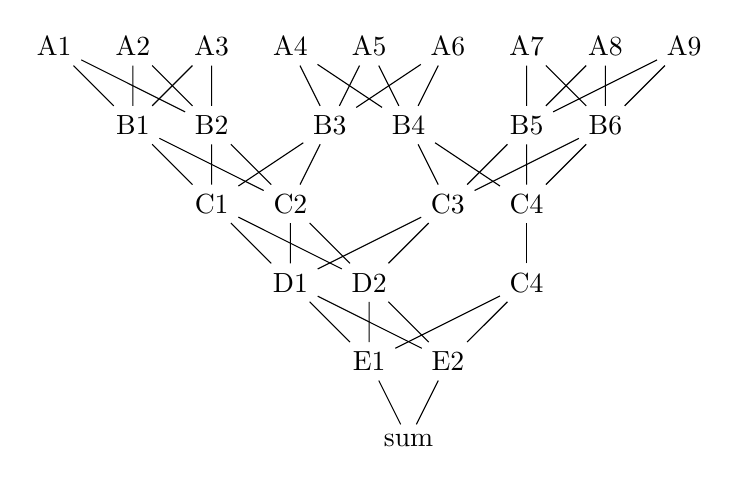
\begin{tikzpicture}
\node (A1) at (0,0) {A1};
\node (A2) at (1,0) {A2};
\node (A3) at (2,0) {A3};
\node (A4) at (3,0) {A4};
\node (A5) at (4,0) {A5};
\node (A6) at (5,0) {A6};
\node (A7) at (6,0) {A7};
\node (A8) at (7,0) {A8};
\node (A9) at (8,0) {A9};

\node (B1) at (1,-1) {B1};
\node (B2) at (2,-1) {B2};
\node (B3) at (3.5,-1) {B3};
\node (B4) at (4.5,-1) {B4};
\node (B5) at (6,-1) {B5};
\node (B6) at (7,-1) {B6};

\draw (B1) --(A1) --(B2);
\draw (B1) --(A2) --(B2);
\draw (B1) --(A3) --(B2);
\draw (B3) --(A4) --(B4);
\draw (B3) --(A5) --(B4);
\draw (B3) --(A6) --(B4);
\draw (B5) --(A7) --(B6);
\draw (B5) --(A8) --(B6);
\draw (B5) --(A9) --(B6);

\node (C1) at (2,-2) {C1};
\node (C2) at (3,-2) {C2};
\node (C3) at (5,-2) {C3};
\node (C4) at (6,-2) {C4};

\draw (C1) --(B1) --(C2);
\draw (C1) --(B2) --(C2);
\draw (C1) --(B3) --(C2);
\draw (C3) --(B4) --(C4);
\draw (C3) --(B5) --(C4);
\draw (C3) --(B6) --(C4);

\node (D1) at (3,-3) {D1};
\node (D2) at (4,-3) {D2};
\node (D3) at (6,-3) {C4};

\draw (D1) --(C1) --(D2);
\draw (D1) --(C2) --(D2);
\draw (D1) --(C3) --(D2);
\draw (D3) --(C4);

\node (E1) at (4,-4) {E1};
\node (E2) at (5,-4) {E2};

\draw (E1) --(D1) --(E2);
\draw (E1) --(D2) --(E2);
\draw (E1) --(D3) --(E2);

\node (sum) at (4.5,-5) {sum};

\draw (E1) --(sum) --(E2);
\end{tikzpicture}

\end{center}

En utilisant la proposition~\ref{reduction_sum} ainsi que le théorème~\ref{cla_sum}, on obtient que la profondeur totale en NAND est majorée par :
\[ 8 \lceil \log_2(s)\rceil + 6+ 12(3p - 2) = 8 \lceil \log_2(s) \rceil + 36p -18.\]
Or, par définition, $p = \lceil \log_3(nb) \rceil$, ce qui permet de conclure.
\end{proof}

\end{subsubsection}
\end{subsection}
\begin{subsection}{Prendre la valeur absolue dans $\ZZq$}
	Rappelons que la valeur absolue d'un élément $x\in \ZZq$ est par définition la valeur absolue de son représentant dans $\rrbracket -q/2, q/2\rrbracket$. 
	
	Dans notre situation, $q = 2^l$ et nous représentons $a\in \ZZq$ par une liste de taille\footnote{pour des raisons techniques, il est en fait représenté par une liste de taille $l$, mais nous ne faisons alors pas attention au dernier bit} $l-1$, le bit de poids faible étant à gauche. Autrement dit :
\[ a = [a_0, ..., a_{l-2}] \quad \text{pour représenter } a = \sum_{i=0}^{l-2} a_i 2^i\]

	On peut alors calculer la valeur absolue de $a$ en binaire ainsi :

\vspace{0.3cm}
\begin{lstlisting}
if $a_{l-2} = 0$: 
	# on a $a < q/2$
	return $a$
else:
	# on a $a \geqslant q/2$, alors $|a - q| = \left( (2^l - 1) - a + 1 \right)$
	$a$ = [NOT($a_i$) for $i$ in range($l$)]
	return cla_sum($a$, $[1,0, ...,0]$)
\end{lstlisting}
\vspace{0.3cm}

Toutefois, nous devons représenter cette algorithme par un circuit booléen et il n'est donc pas possible de faire de
conditions. On va donc considérer la modification du code suivante:

\vspace{0.3cm}
\begin{lstlisting}
$b$ = cla_sum([$\overline{a_i}$ for $i$ in range($l$)], $[1,0, ...,0]$ )
return [($a_{l-1} \land a_i) \lor (\overline{a_{l_1}} \land b_i)$  for $i$ in range($l$)]
\end{lstlisting}
\vspace{0.3cm}

Notre algorithme a encore un dernier problème: il n'est pas possible d'utiliser des constantes
dans notre circuit booléen, on ne peut donc à priori pas faire l'instruction

\vspace{0.3cm}
\begin{lstlisting}
$b$ = cla_sum([$\overline{a_i}$ for $i$ in range($l$)], $[1,0, ...,0]$ )
\end{lstlisting}
\vspace{0.3cm}
Notons toutefois que pour un booléen $x$
\[\overline{x \wedge 0 } = x \qquad \overline{x \wedge 1 } = \overline{x}\]
Il est donc possible de remplacer tout NAND avec une  constante par une opération sans constante
ayant une profondeur de NAND inférieur ou égale. \\
On peut donc se passer de cette constante, et le calcul de profondeur que l'on effectue avec cette constante
majore celui qu'on aurait fait en s'en passant.

\paragraph{}
Utilisons le théorème \ref{cla_sum} pour conclure:
\begin{prop}
Il est possible de calculer la valeur absolue en binaire d'un élément $a\in \ZZq$ avec une profondeur de moins de
$8\lceil \log_2(s) \rceil + 11$ NAND.
\end{prop}
\end{subsection}

Maintenant que nous avons étudié comment sommer des listes et comment calculer la valeur absolue dans
$\ZZq$, nous pouvons déterminer une majoration du nombre de NAND nécessaire pour appliquer l'algorithme
de déchiffrement tel que décrit dans le listing~\ref{lst:decoupage} page~\pageref{lst:decoupage}.
\begin{thm} \label{size_dec}
Si $q$ est une puissance de 2, on peut effectuer 
l'algorithme \textbf{Decrypt} avec une profondeur de NAND plus petite que
\[88 \lceil \log_2(\log_2(q)) \rceil + 36 \lceil \log_2(n) \rceil \]
et donc, en $\mathcal{O}(\log_2(n) + \log_2(\log_2(q)))$
\end{thm}
\begin{proof}
En utilisant les propositions précédentes ainsi que le fait qu'il y a au plus $N*l = \log_2(q)^2 * (n+1)$ listes à
sommer, on majore la profondeur de NAND par
\[16 \lceil \log_2(\log_2(q)) \rceil + 36 \log_3\left(\log_2(q)^2
*(n+1)\right) = 16 \lceil \log_2(\log_2(q)) \rceil + 72 \lceil \log_3(\log_2(q)) \rceil + 36 \lceil \log_3(n+1) \rceil \]
et on majore le logarithme en base 3 par celui en base 2 pour conclure, en
utilisant aussi que $\log_3(n+1) \leqslant\log_2(n)$ (dès $n \geqslant 2)$.
\end{proof}

Nous avons maintenant toutes les informations nécessaires pour choisir des paramètres permettant le bootstrapping.

\begin{subsection}{Choix asymptotique de paramètres pour GSW avec bootstrapping}
\label{sec:bootstrapping}

On va utiliser l'inégalité grossière :
\[88 \lceil\log_2(\log_2(q))\rceil + 36 \log_2(\log_2(n)) \leqslant 90\left(\log_2(\log_2(q)) + \log_2(n)\right) \]
pour voir que, pour obtenir un GWS avec bootstrapping, il suffit de pouvoir évaluer les circuits dont la profondeur en NAND est majorée par
\[ L = 90 \left(\log_2(\log_2(q)) + \log_2(n)\right). \]
L'inégalité est assez grossière pour qu'on n'ait pas besoin de rajouter de 1 à la profondeur maximale pour s'assurer de pouvoir effectuer des calculs hors de ce circuit.

\paragraph{}
On a vu dans la section \ref{param_leveled} que pour avoir une
profondeur de $L$ NAND, il suffit d'avoir
\begin{equation*}
q > 16 {(1+N)}^{L+2}.
\end{equation*}
En injectant la valeur précédente dans $L$ et en utilisant une majoration
grossière, on voit qu'il suffit d'avoir
\begin{equation}
q > {\left((n+1)(\lceil \log_2(q) \rceil + 1 )\right)}^{90 \left(\log_2(n) +
\log_2(\log_2(q))\right)}.
\end{equation}

Suivant le raisonnement de Shai Halevi dans \cite{halevi}, on remarque 
qu'il existe un $\rho > 90$ tel que 

\begin{equation*}
{\left((n+1)(\lceil \log_2(q) \rceil + 1 )\right)}^{90 \left(\log_2(n) +
\log_2(\log_2(q))\right)} < 
{\left(n\log_2(q))\right)}^{\rho\:\left(\log_2(n) + \log_2(\log_2(q))\right)}.
\end{equation*}
En utilisant l'hypothèse  \ref{hyp_dlwe_boot} (page \pageref{hyp_dlwe_boot}), notre jeu de contraintes est alors:

\[ \begin{cases}
\alpha  = n /q \\
	q = 2^\text{polylog$(n)$}\\ 
	m = 2(n+1) \bnorm{q} \\  
	q > {\left(n\log_2(q))\right)}^{\rho\: \left[\log_2(n) + \log_2(\log_2(q))\right]}
	\end{cases} \]

\paragraph{}
Cela nous amène à un choix de paramètres:
\begin{thm}{Paramètres sécurisés pour GSW avec bootstrapping}

Nous gardons les notations précédentes.
Sous l'hypothèse de sécurité circulaire ainsi que l'hypothèse \ref{hyp_dlwe_boot} de difficulté de DWLE, les paramètres
suivants rendent le cryptosystème GSW bootstrappable et IND-CPA :

\[ \begin{cases}
 	n = \lambda \\
	q = \lceil n^{\rho \log^2(n)}\rceil \\
	m = 2(n+1) \bnorm{q} \\  
	\alpha = n/q = 2^{\Theta(\log^2(n))}
	\end{cases} \]
\end{thm}
\begin{proof}
Il nous faut montrer que l'inégalité 
	\[ q > {\left(n\log_2(q)\right)}^{\:\rho\:\left(\log_2(n) + \log_2(\log_2(q))\right)} \]
est vérifiée pour $n$ assez grand.

\paragraph{}
En substituant $q$ par sa valeur à gauche, l'inégalité devient:
\begin{equation*}
n^{\rho \log^2(n)} > {\left(n\log_2(q))\right)}^{\:\rho\: \left(\log_2(n) + \log_2(\log_2(q)\right)}.
\end{equation*}

En passant au logarithme, l'inégalité devient:
\[ \log^3(n) > {\left[\log_2(n) + \log_2(\log_2(q))\right]}^2. \]

Or,
\[ \log_2(\log_2(q)) \leqslant \log_2(\rho \log^3(n) + 1) \leqslant 1 + \log_2(\rho) + 3 \log_2(\log_2(n)).\]
Il suffit donc de montrer que:
\[ \log^3(n) > {(1 + \log_2(\rho) + 3\log_2(\log_2(n)) + \log_2(n))}^2,\]
ce qui est vrai pour $n$ assez grand.
\end{proof}
\begin{rmq}
Notons que dans notre première tentative, avec \textbf{basic\_sum} à la place de \textbf{cla\_sum}, 
les contraintes obtenues étaient impossibles à respecter.
\end{rmq}

\paragraph{}
La figure~\ref{size_boostrapping} nous montre la taille nécessaire
pour stocker les différents composants de GSW en utilisant ces paramètres.
On voit qu'elles sont irréalistes.
\begin{figure}[!ht]
\begin{tabular}{|l|c|c|c|}
\hline
& taille de pk & taille de sk& taille d'un chiffré \\
\hline
$\lambda = 8, \ \rho = 90$ & 3 Ko & 113 Mo & 135 Go \\
\hline
$\lambda = 8, \ \rho = 100$ & 3 Ko & 139 Mo & 186 Go \\
\hline
$\lambda = 16, \ \rho = 90$ & 12 Ko & 2 Go & 6 To \\
\hline
$\lambda = 16, \ \rho = 100$ & 13 Ko & 3 Go & 9 To \\
\hline
$\lambda = 32, \ \rho = 90$ & 45 Ko & 32 Go & 176 To \\
\hline
$\lambda = 32, \ \rho = 100$ & 50 Ko & 40 Go & 242 To \\
\hline
\end{tabular}
\caption{Taille des données suivant les paramètres étudiés précédemment}
\label{size_boostrapping}
\end{figure}

\end{subsection}
\end{section}
